{\color{gray}
All images and additional material go there.
}

\subsection{Benefits of microservices}
\label{app:ms-benefit}

To understand the benefits and motivations behind using \gls{ms} over
the monolithic style, we will first look at the latter.
\cite{ms-definition}

Monolithic architectures build applications using a single unit. This
basically means that all of an application's functionality, logic,
classes, function and name spaces are in the end located within a
single executable and thus run within a single process.
\cite{ms-definition} This model is very much usable in fact and allows
us to create functioning systems---as has demonstrated the time of
software development before \glspl{ms} were introduced. However, this
architectural style raises some issues nonetheless. For instance, even
the smallest of changes in an application require the whole product to
be rebuilt and redeployed or redistributed which is not necessarily
ideal in the case of large applications with multiple end-users.

As the application's life cycles goes on, it is unavoidable to modify
it over time. In a monolithic system however, it becomes increasingly
difficult to maintain a modular structure---if one was present to
begin with---which in turn also leads to modifications becoming more
expensive. \cite{ms-definition} The expensive modifications are
explained by the fact that if a modular structure cannot be
guaranteed, it possibly entails that changes to one component may
impact other components which were not supposed to be affected.
\cite{ms-definition} This may result in many adjacent changes and
unexpected issues to be performed and treated respectively.

Lastly, if we want to scale an application we actually need to scale
the application as a whole rather than the individual components that
need to be scaled.

\begin{figure*}
	\centering
	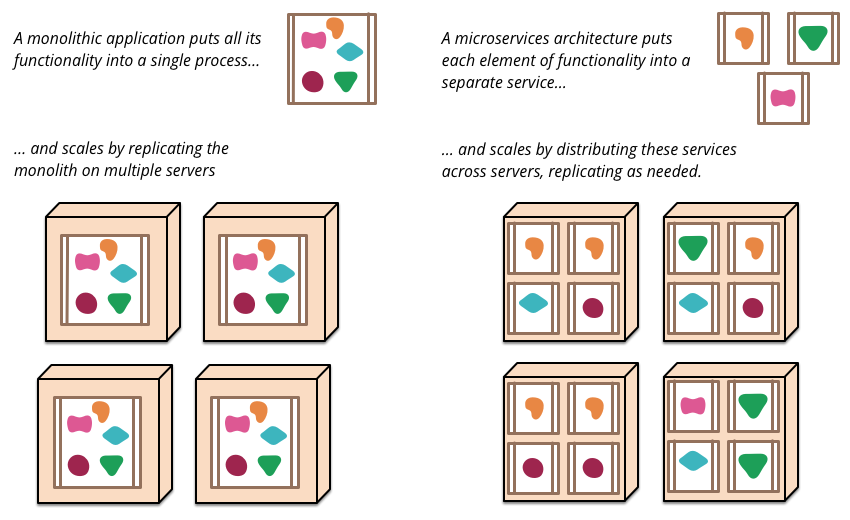
\includegraphics[width=0.75\linewidth]{images/sketch.png}
	\caption{Monoliths and Microservices \cite{ms-definition}}
	\label{fig:monoliths-ms}
\end{figure*}

Figure \ref{fig:monoliths-ms} nicely demonstrates some of the
aforementioned issues and how the \gls{ms} architecture tries to
tackle them.

Since the application is now split into separate services, making
modifications will not require us to build and deploy the whole
application anew. It will be enough to only update the services in
question.

Further, the fact that the application is built in a modular fashion
from the ground up and divided into smaller chunks and services makes
it easier to maintain a modular structure within the application as a
whole. As a result, making changes to one such service will guarantee
that none of the other services will be affected and thus keep
undesired or unforeseen side effects to a minimum.

We can also see that scaling an application becomes much less of a
burden. No longer do we need to scale the whole application, but we
can simply introduce new services where needed.


\subsection{Obtaining data from E4L}
\label{app:e4l-data}

To give an outline, our first attempt was to sort of brute-force our
way into obtaining data. While not the most useful of data, it was
something to work with. Only later have we discovered that \gls{e4l}
exposes an API which greatly alleviates the burden of our brute-force
approach.

Obtaining useful data however, was only achievable thanks to the help
and guidance of a prior team member of \gls{e4l} who had great
responsibility in creating the back-end. He showed me the proper way to
obtain all the data from the API as well as by directly connecting to
the \gls{e4l} database.

\paragraph{First attempt at obtaining data from the back-end}

Upon inspection of the \gls{e4l} backend, we were able to find a
potentially relevant endpoint that would allow us to query answers
from the questionnaire.  However, it quickly became apparent that the
back-end endpoints were specifically made to be used by the front-end
page. Further evidence for this can be found in the functionalities
described in the README, which also informs us that the only data that
can be extracted is specific to a session. All of this essentially
means that we have no direct way to access any data beyond what we are
presented with on the web page---which would only comprise our results
from after answering the questionnaire.

Upon completing the questionnaire in E4L, we are presented the
following page\footnote{Note that the ID will be different. This is an
example for a results page that we obtained at some point.}:
\url{https://juno.uni.lux/e4l/result/MzA5.-7-sMYXmv3tXyuLQT2s1ZgULRKY}.
The so-called	\textit{sessionId} is unique to our provided answers, so
by taking note of it we are able to review our \textit{energy scores}
at any point in time. The obvious course of action now would be to use
the \verb|/calculate/session/{sessionId}| endpoint---which is our only
of two GET handlers regarding the questionnaire---to obtain our
results.

One problem rose quickly however: We had no information on where or
how to access the back-end in order to issue our GET request. Upon
inspection in the code for both the front-end and back-end, we were
unable to find any concrete traces on how to reach it. The closest we
managed to find was the definition of a \verb|baseUrl| using \verb|axios|,
but that still left us clueless. So we set out to create a web scraper
that would parse the HTML of the above results page.

\paragraph{Scraping the results page for data}

We used \verb|selenium| to perform this task. However, running the
selenium browser in headless mode---as is required for running this
code in a docker container---caused issues with our scraper. It turns
out that the page contents would not be loaded unless the page was
actually rendered by the browser. In addition to this approach being
extremely slow due to \verb|selenium|, it was simply not usable for
our use-case.

\paragraph{Obtaining data from the back-end API}

It was only after a third and final inspection of the E4L
code---performed while documenting what we did---with the help of
GitLab's search utility, that we discovered how to access the
back-end.  It was hidden in plain site in the front-end README,
however it was not emphasised very well which caused us to completely
overlook it at multiple occasions.

That said, we were able to retrieve our results using the API by
issuing a GET request on
\\\url{https://juno.uni.lux/e4lapi/calculate/session/MzA5.-7-sMYXmv3tXyuLQT2s1ZgULRKY}.
However, some data about global statistics (i.e. Luxembourg, Europe,
World) were not available as they seemed to be hard coded into the
front-end.

\paragraph{Obtaining all the data by querying the API and database}

This step is elaborated on in the technical production section
\ref{sec:e4l-data-query}
